\documentclass[bwprint]{gmcmthesis}
\usepackage[framemethod=TikZ]{mdframed}
\begin{document}

\newpage
%附录
\appendix
% \setcounter{page}{1} %如果需要可以自行重置页码。
\newpage
\section{数据预处理及读取函数}\label{数据预处理及读取函数}
\section{问题一主程序}
\section{问题一FFFD算法}\label{问题一FFFD算法}
\section{问题二主程序}
\section{问题二FFFD算法}
\section{问题二材质订单排序算法}
\newpage
\section{问题一dataA1排样方案}
\begin{figure}[!htbp]
    \centering
    \begin{minipage}{0.1\linewidth}
        \centering
        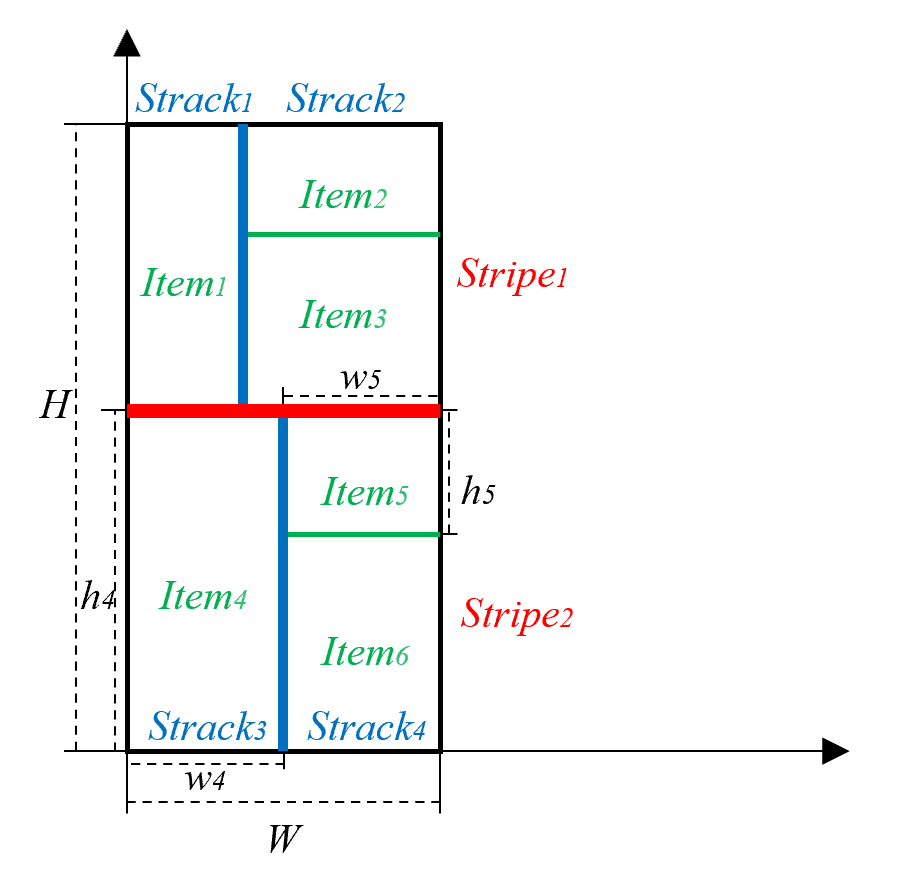
\includegraphics[width=.9\textwidth]{方向说明1.png}
    \end{minipage}
    \begin{minipage}{0.1\linewidth}
        \centering
        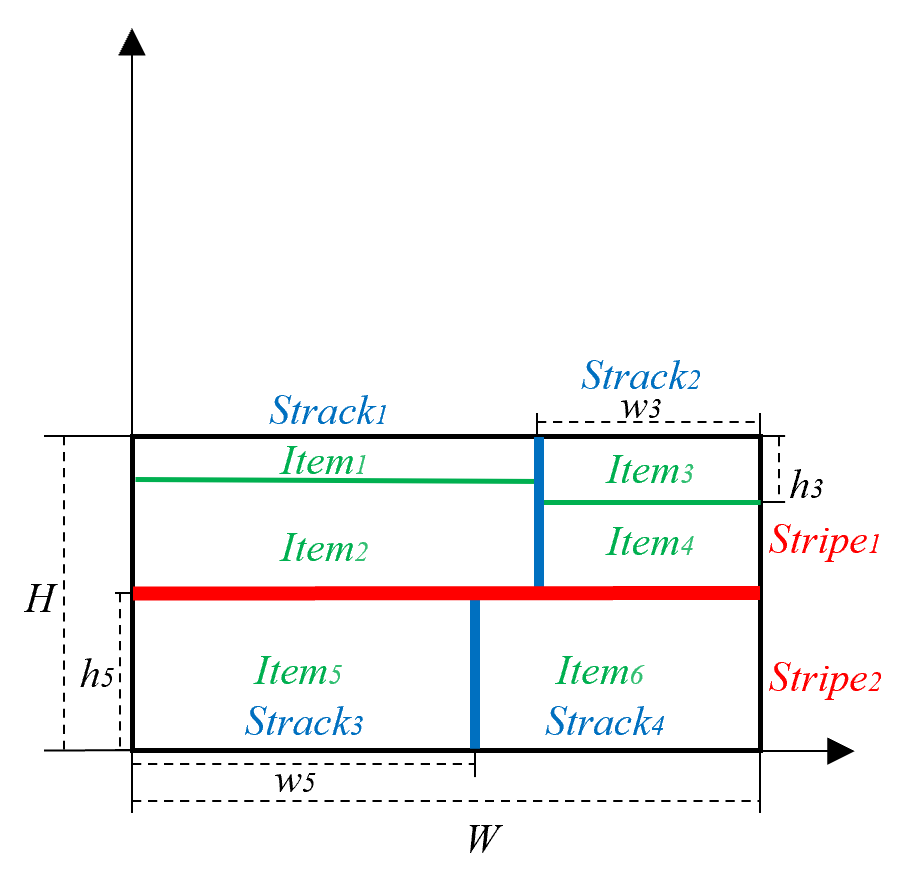
\includegraphics[width=.9\textwidth]{方向说明2.png}
    \end{minipage}
    \begin{minipage}{0.1\linewidth}
        \centering
        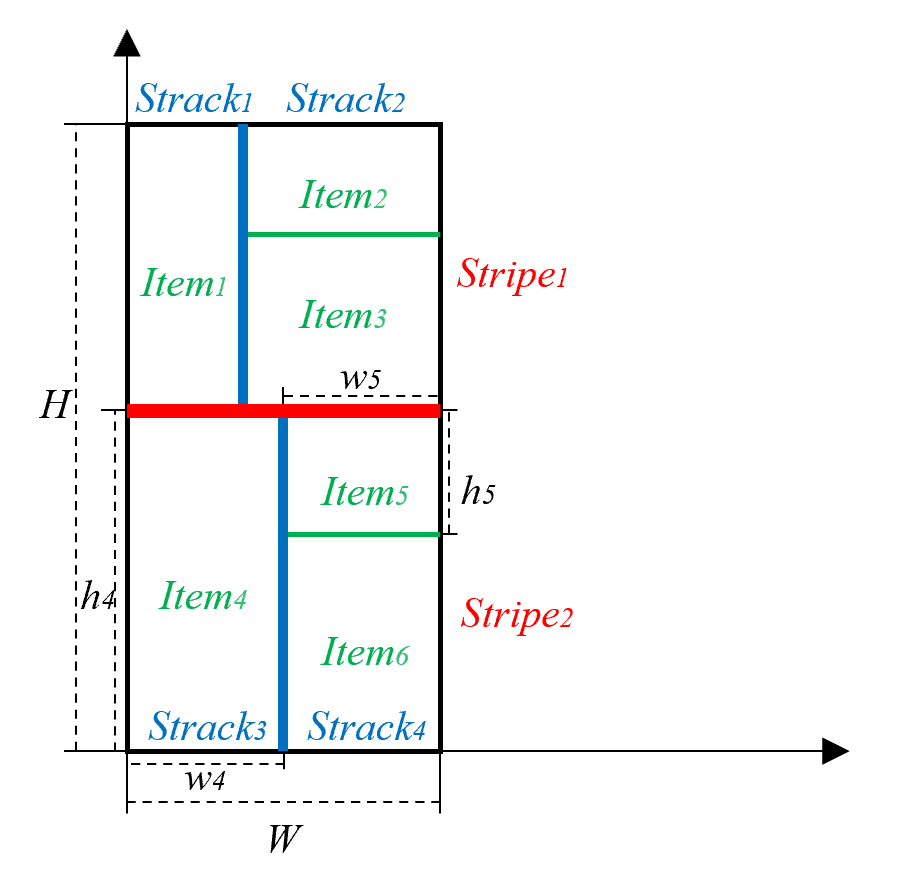
\includegraphics[width=.9\textwidth]{方向说明1.png}
    \end{minipage}
    \begin{minipage}{0.1\linewidth}
        \centering
        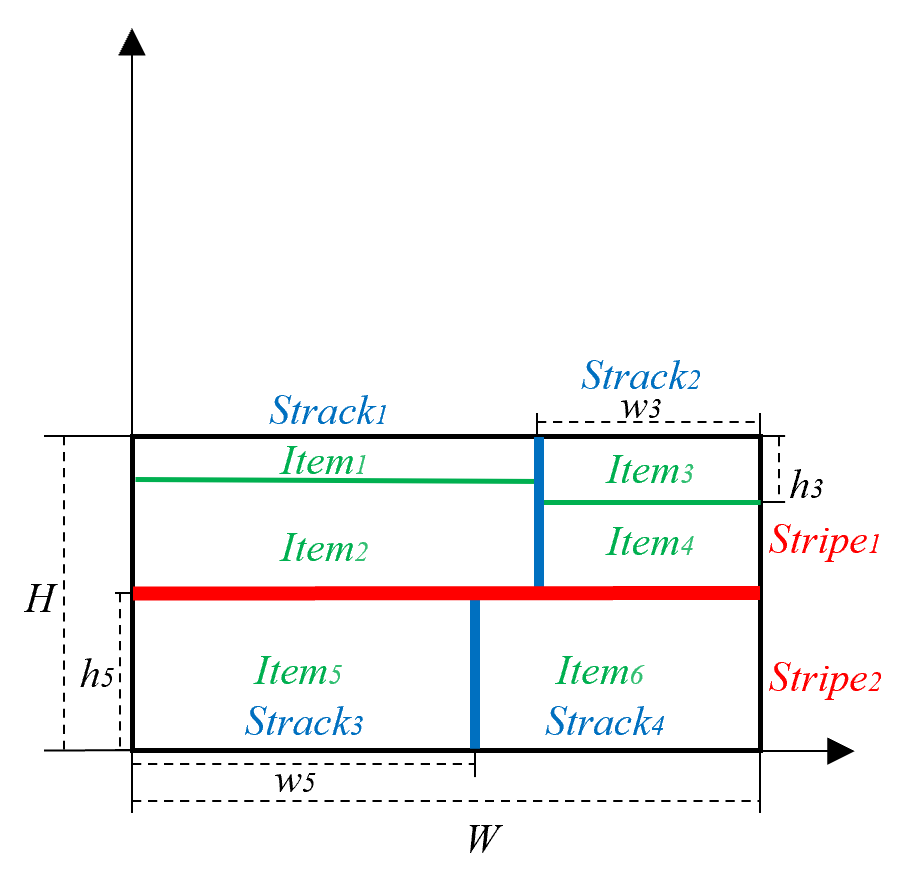
\includegraphics[width=.9\textwidth]{方向说明2.png}
    \end{minipage}
    \begin{minipage}{0.1\linewidth}
        \centering
        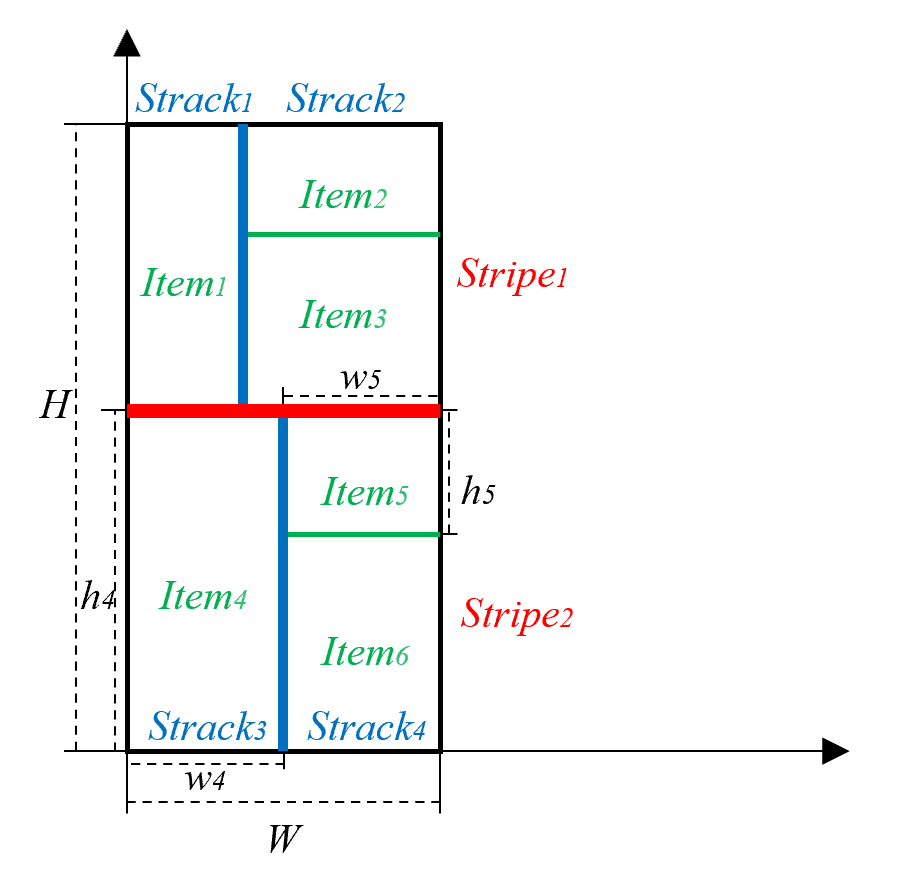
\includegraphics[width=.9\textwidth]{方向说明1.png}
    \end{minipage}
\end{figure}
\begin{figure}[!htbp]
    \centering
    \begin{minipage}{0.1\linewidth}
        \centering
        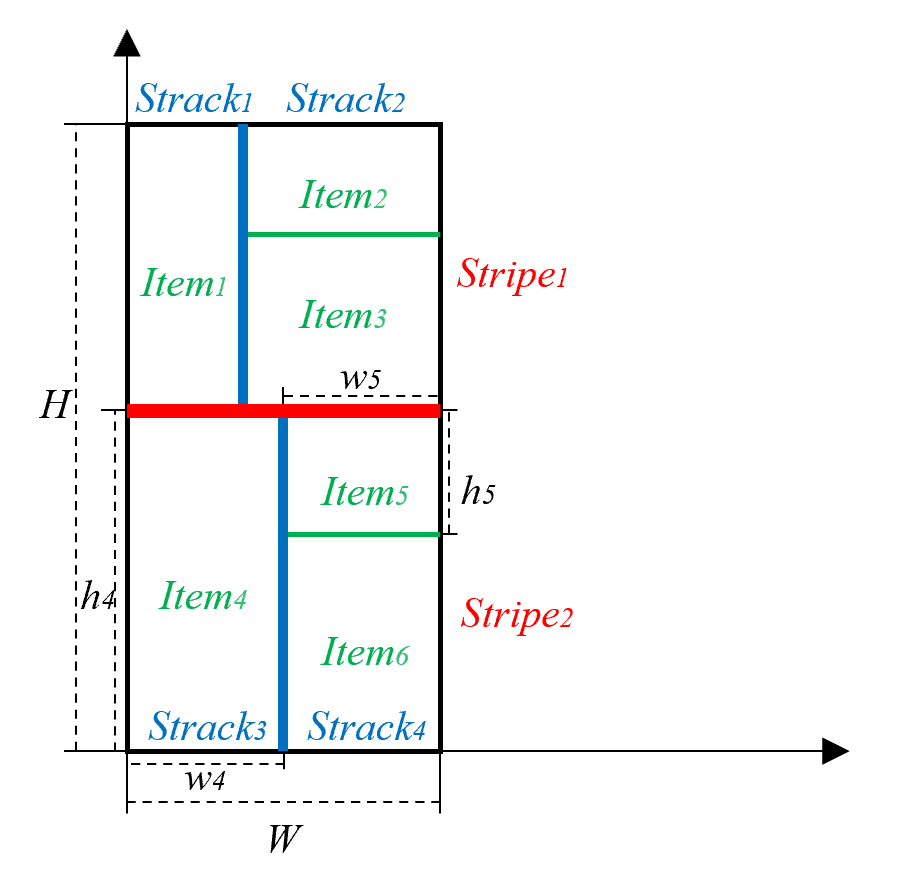
\includegraphics[width=.9\textwidth]{方向说明1.png}
    \end{minipage}
    \begin{minipage}{0.1\linewidth}
        \centering
        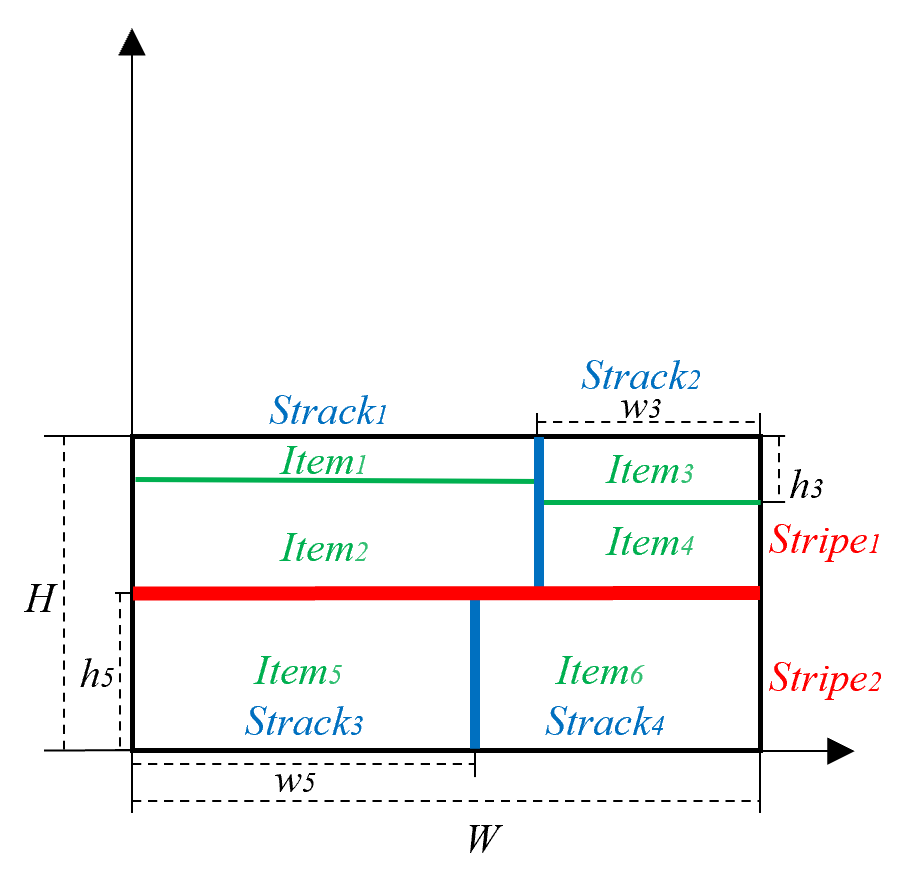
\includegraphics[width=.9\textwidth]{方向说明2.png}
    \end{minipage}
    \begin{minipage}{0.1\linewidth}
        \centering
        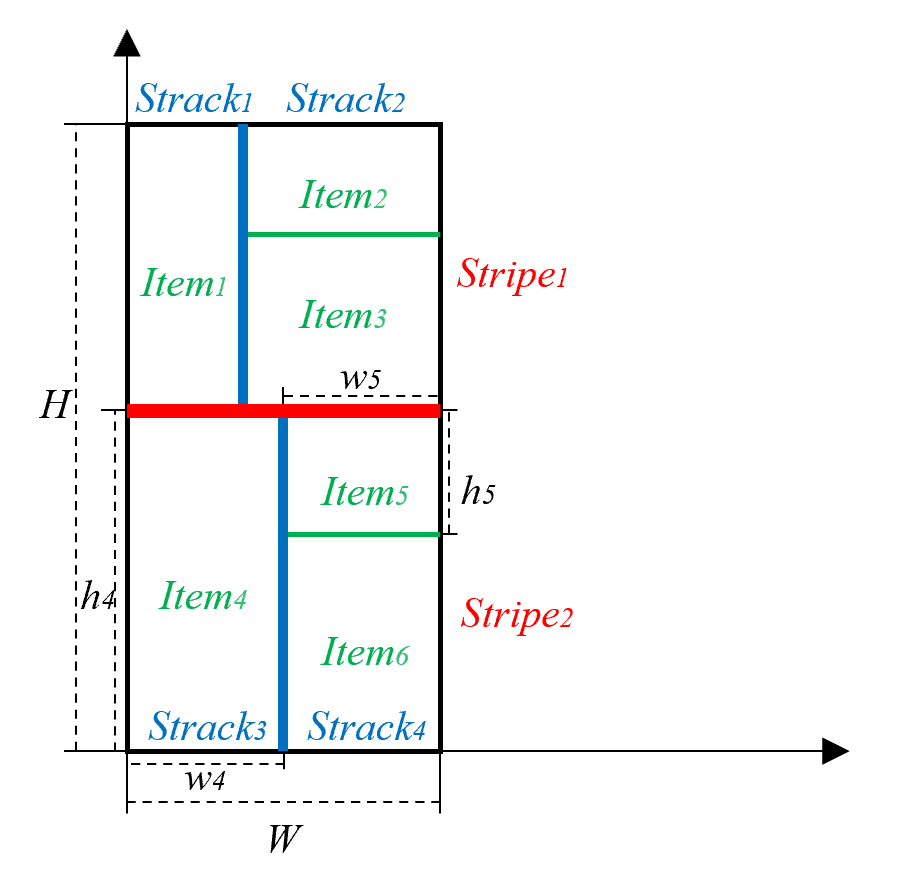
\includegraphics[width=.9\textwidth]{方向说明1.png}
    \end{minipage}
    \begin{minipage}{0.1\linewidth}
        \centering
        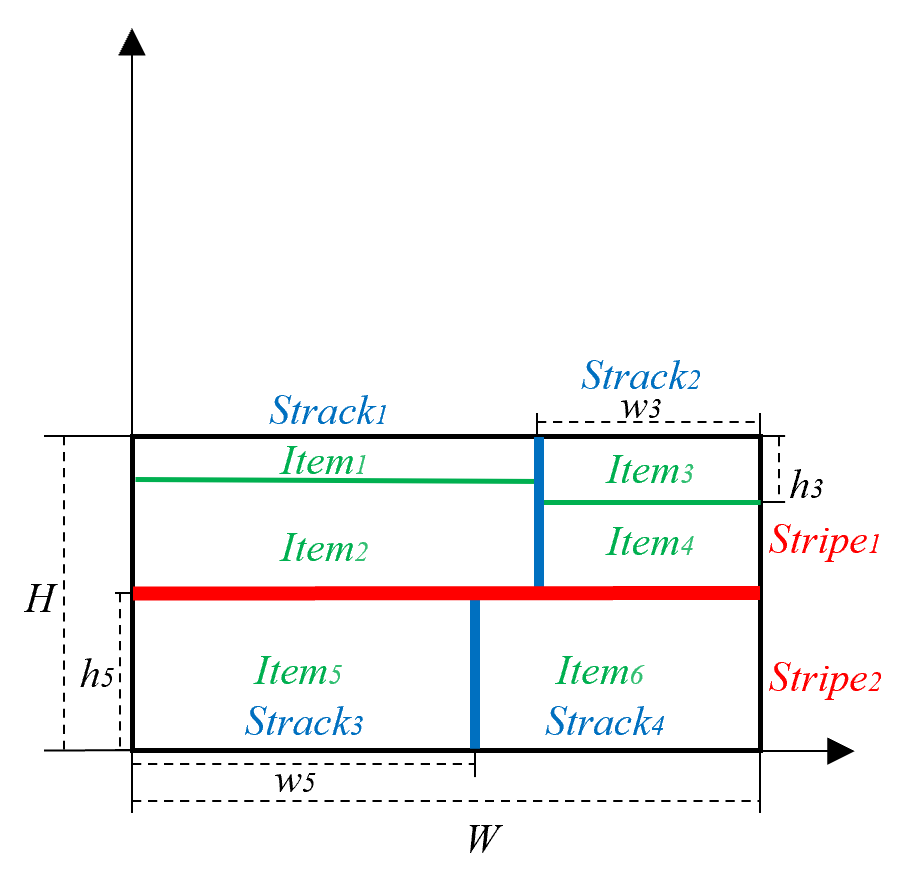
\includegraphics[width=.9\textwidth]{方向说明2.png}
    \end{minipage}
    \begin{minipage}{0.1\linewidth}
        \centering
        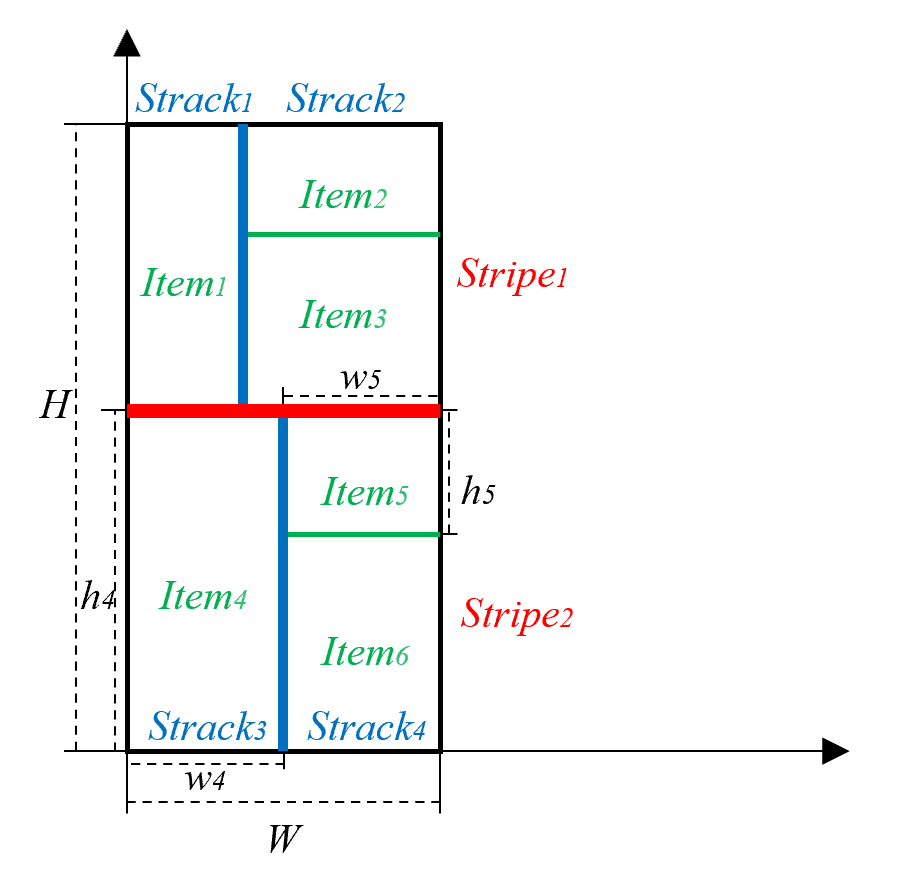
\includegraphics[width=.9\textwidth]{方向说明1.png}
    \end{minipage}
\end{figure}
\end{document} 